% %%%%%%%%%%%%%%%%%%%%%%%%%%%%%%%%%%%%%%%%%%%%%%%%%%%%%%%%%%%
% Hier nichts aendern
\documentclass[sigconf, nonacm, review]{acmart}
\AtBeginDocument{%
  \providecommand\BibTeX{{%
    \normalfont B\kern-0.5em{\scshape i\kern-0.25em b}\kern-0.8em\TeX}}}

\setcopyright{acmcopyright}
\copyrightyear{2018}
\acmYear{2018}
\acmDOI{XXXXXXX.XXXXXXX}
\acmJournal{JACM}
\acmVolume{37}
\acmNumber{4}
\acmArticle{111}
\acmMonth{8}
\acmPrice{15.00}
\acmISBN{978-1-4503-XXXX-X/18/06}
% Hier nichts aendern
% %%%%%%%%%%%%%%%%%%%%%%%%%%%%%%%%%%%%%%%%%%%%%%%%%%%%%%%%%%%

\begin{document}
% %%%%%%%%%%%%%%%%%%%%%%%%%%%%%%%%%%%%%%%%%%%%%%%%%%%%%%%%%%%
% Hier eigene Daten eingeben
\title{Report zum Fachprojekt Routingalgorithmen}
\author{Pouria Araghchi}
\affiliation{%
  \institution{TU Dortmund}
  \streetaddress{Otto-Hahn-Straße 14}
  \city{Dortmund}
  \country{Deutschland}}
\email{pouria.araghchi@tu-dortmund.de}

\author{Kai Lukas Ilmenau}
\affiliation{%
  \institution{TU Dortmund}
  \streetaddress{Otto-Hahn-Straße 14}
  \city{Dortmund}
  \country{Deutschland}}
\email{kai.ilmenau@tu-dortmund.de}

\author{Naveed Niazi}
\affiliation{%
  \institution{TU Dortmund}
  \streetaddress{Otto-Hahn-Straße 14}
  \city{Dortmund}
  \country{Deutschland}}
\email{naveed.niazi@tu-dortmund.de}

\renewcommand{\shortauthors}{Araghchi, Ilmenau, Niazi}
% Hier eigene Daten eingeben
% %%%%%%%%%%%%%%%%%%%%%%%%%%%%%%%%%%%%%%%%%%%%%%%%%%%%%%%%%%%

\begin{abstract}
In der heutigen Zeit werden mehrere Millionen Datenpakete von und zu Knotenpunkten verschickt.
Daher ist das \emph{Routing} von diesen Datenpaketen in der heutigen Zeit wichtiger denn je.
Gutes Routing kann Datenstaus verringern oder sogar verhindern, Verteilerknoten auslasten oder entlasten 
und sorgt damit fuer einen reibungslosen Datenverkehr ueberall auf der Welt.
Wie gut das Routing innerhalb einer Netzwerktopologie ist, wird durch den darunterliegenden Routingalgorithmus bestimmt.
Hierf\"ur gibt es verschiedenste Ans\"atze mit variierender Komplexit\"at und Erfolgswahrscheinlichkeit.
\end{abstract}

\begin{CCSXML}
<ccs2012>
<concept>
<concept_id>10003033.10003068.10003073.10003076</concept_id>
<concept_desc>Networks~Traffic engineering algorithms</concept_desc>
<concept_significance>500</concept_significance>
</concept>
</ccs2012>
\end{CCSXML}

\ccsdesc[500]{Networks~Traffic engineering algorithms}

% Eventuell keywords weglassen
\keywords{weight optimization, waypoint optimization}

\received{6. August 2023}
\received[\"uberarbeitet]{\textcolor{red}{ausstehend}}
\received[akzeptiert]{15. August 2023}

\maketitle

\section{Einleitung}
\textcolor{red}{fehlt}

\section{Theoretische Grundlagen}
\textcolor{red}{Hier wird etwas zum Paper stehen}\cite{foerster2021}.
\section{Umsetzung}
In diesem Abschnitt werden unsere Projekte und die dazugeh\"origen Ideen vorgestellt.
Die beiden Projekte sind in Unterabschnitte und die algorithmischen Ideen und Umsetzungen des jeweiligen Gruppenmitglieds in Paragraphen unterteilt. 
\subsection{Algorithmen zu Projekt 1}
In Projekt 1 ging es darum, eine algorithmische Idee auf Basis von \cite{foerster2021} herauszuarbeiten und diese mithilfe desselben Git-Prokjekts\footnote{\url{https://github.com/fruitiestPunch/FaPro_P1}, siehe Abschnitt \ref{sec:resouces}} mit alternativen Routingalgorithmen zu vergleichen. 
\subsubsection{Sequential combination aus inverse capacity und demand first waypoints}
Der Kerngedanke hier war es, einen einen schnellen Algorithmus zu finden, 
welcher hinreichend gute Ergebnisse in Bezug auf die MLU abliefert.
Diese Eigenschaft ist insbesondere f\"ur Netzwerke sinvoll,
dessen Auslastungen sich regelm\"a\ss ig w\"ahrend des Betriebs \"andern und der ALgorithmus reaktiv sehr schnell alle Gewichte und Wegpunkte neu berechnet.
Die Grundlage dieses Algorithmus war die sequentielle Kombination von dem empirisch h\"aufig verwendetem $inverse\_capacity$ und dem etwas langsameren aber genaueren $demand\_first\_waypoints$.
\emph{Anmerkung: Die Algorithemn Namen "demand first waypoints" und "greedy waypoints" sind hier austauschbar.}\newline
Daraufhin bildeten sich zwei Fragen.
\begin{enumerate}
    \item Ist die Kombination genauer als dessen Bestandsteile?
    \item Ist die zus\"atzliche Rechenzeit gerechtfertigt?
\end{enumerate}
% Das [h] kann weg, dann findet Tabelle automatisch den besten Platz
\begin{figure}
\centering
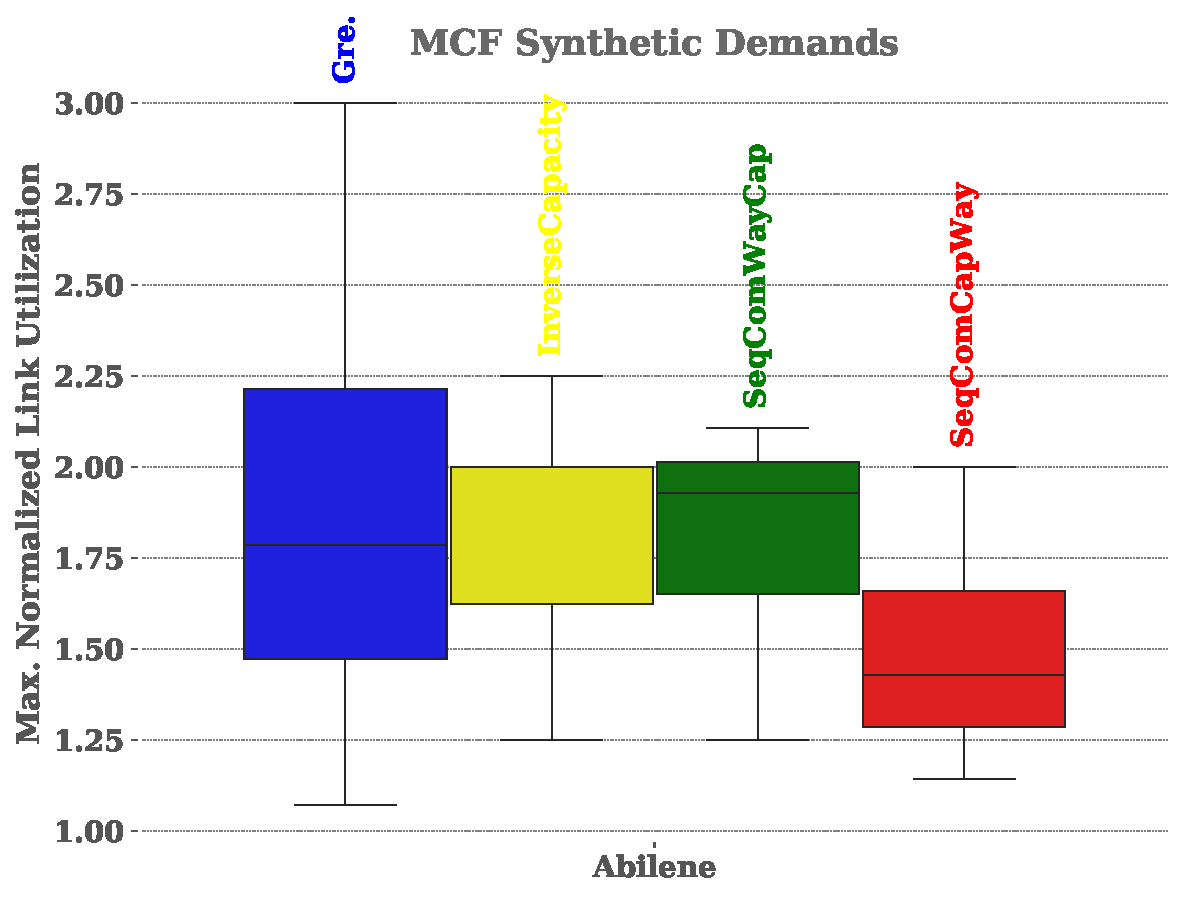
\includegraphics[width=\linewidth]{figures/pouria_all_algorithms_abilene.pdf}
\caption{Vergleich von vier Algorithmen mit syntetischen Anforderungen auf der Abilene-Topologie. Legende: greedy waypoints in blau, inverse capacity in gelb, SeqComWayCap in gr\"un, SeqComCapWay in rot.}
\label{fig:pouriaBoxplotSynthetic}
\end{figure}
% Das [h] kann weg, dann findet Tabelle automatisch den besten Platz
\begin{figure}
\centering
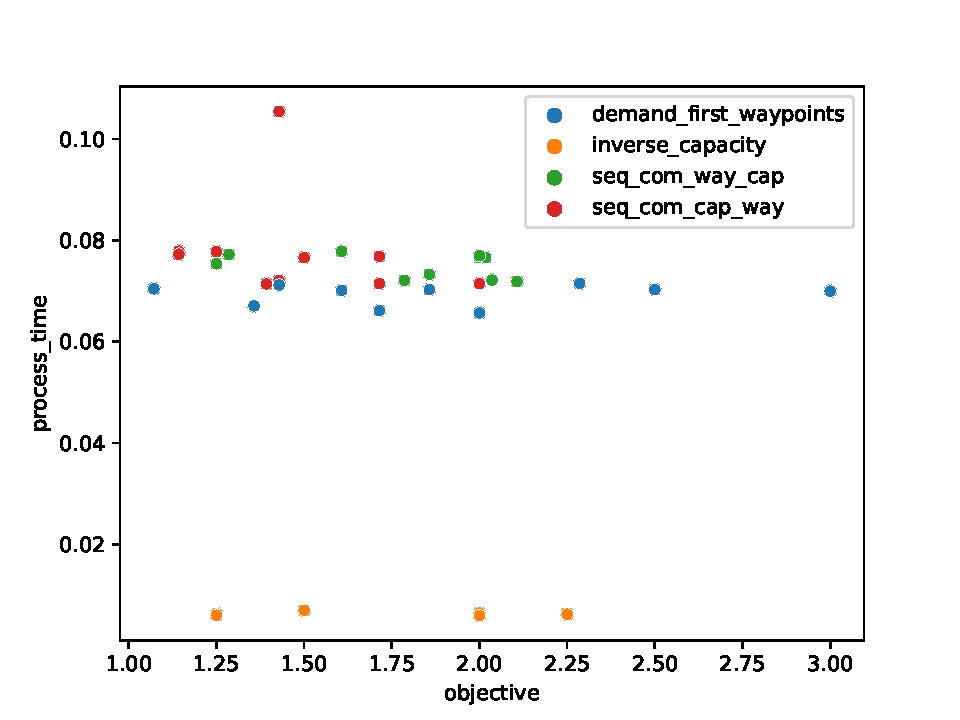
\includegraphics[width=\linewidth]{figures/pouria_colored_scatter_plot_results_all_algorithms.pdf}
\caption{Vergleich von vier Algorithmen mit syntetischen Anforderungen auf der Abilene-Topologie. Legende: greedy waypoints in blau, inverse capacity in gelb, SeqComWayCap in gr\"un, SeqComCapWay in rot.}
\label{fig:pouriaScatterSynthetic}
\end{figure}
Die Abbildungen \ref{fig:pouriaBoxplotSynthetic} und \ref{fig:pouriaBoxplotReal} zeigen, 
dass die sequentielle Kombination beider Algorithmen in beiden F\"allen mindestens genauso gut ist wie eines seiner Bestandteile. 
Im Fall von $SeqComCapWay$ ist dieser im Durchschnitt sogar besser als beide Algorithmen.
Dies l\"asst sich darauf zur\"uckf\"uhren, 
dass die Kantengewichte durch den Algorithmus $inverse\_capacity$ zu Beginn verbessert werden 
und anschlie\ss end durch den zweiten Algorithmus weiter verbessert werden, falls m\"oglich.
\subsection{Experimente zu Projekt 2}
In diesem Projekt ging es darum, die eigene algorithmische Idee zu nehmen und in einem virtuellen Netzwerk\footnote{\url{https://github.com/nikolaussuess/nanonet}, siehe Abschnitt \ref{sec:resouces}} zu testen. 
Dieses Projekt wurde ebenfalls mithilfe eines bereits existierenden Repositories\footnote{\url{https://github.com/fruitiestPunch/FaPro_P2}, siehe Abschnitt \ref{sec:resouces}} bearbeitet.
\subsubsection{Sequential combination aus inverse capacity und demand first waypoints}
\label{sec:seq_com_p2}
Zum Testen dieses Algorithmus wurde eine vereinfachte Topologie mit wenigen Anforderungen erstellt.
In Abbildung \ref{fig:pouriaSimpleTopology} ist die finale Topologie zu sehen, 
wobei hier bereits der $inverse\_capacity$-Algorithmus darauf ausgef\"uhrt wurde.
In der Tabelle \ref{tab:pouriaSimpleTopology} sind die beiden Anforderungen sowie deren Start- und Endknoten angegeben.
Die Timeouts in diesen Experimente haben zu einigen Problemen gef\"uhrt.
Da der Rechner auf dem speziell dieser Algorithmus getestet wurde,
relativ schwach war (4GB RAM), wird vermutet, 
dass die Timeouts
\footnote{\url{https://github.com/nikolaussuess/nanonet}, siehe Abschnitt \ref{sec:resouces}}
\footnote{\emph{nanonet\_batch.py} aus \url{https://github.com/fruitiestPunch/FaPro_P2}, siehe Abschnitt \ref{sec:resouces}}
\begin{verbatim}
  at now+2min
\end{verbatim}
und 
\begin{verbatim}
  sleep(8 * 60)
\end{verbatim}
nicht ausgereicht haben, sodass einige der Prozesse fr\"uhzeitig abgerbochen wurden.
Abbildung \ref{fig:pouria_boxplot_no_boxes} zeigt dabei die MLU-Werte aller drei Algorithmen im Vergleich.
Die Tatsache, dass die Boxplots hier nur als Striche dargestellt werden, weist daraufhin, dass es keine Streuung in den finalen Ergebnissen gab,
was auf das fr\"uhzeitige Abbrechen einiger Rechenprozesse zur\"uckgef\"uhrt werden kann.
\begin{figure}
\centering
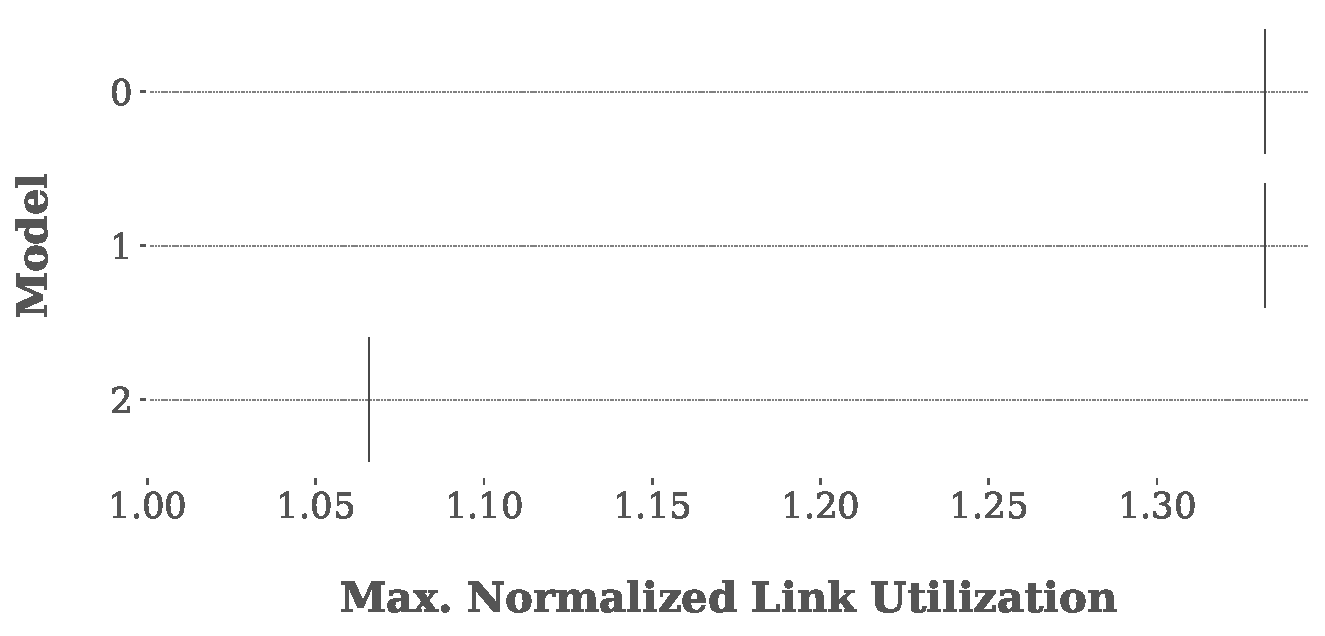
\includegraphics[width=\linewidth]{figures/pouria_boxplot_no_boxes.pdf}
\caption{Vergleich von drei Algorithmen als Boxplotdiagramme. Legende: 0 = Joint, 1 = Weights, 2 = Pouria.}
\label{fig:pouria_boxplot_no_boxes}
\end{figure}
% Das [h] kann weg, dann findet Tabelle automatisch den besten Platz
\begin{figure}
\centering
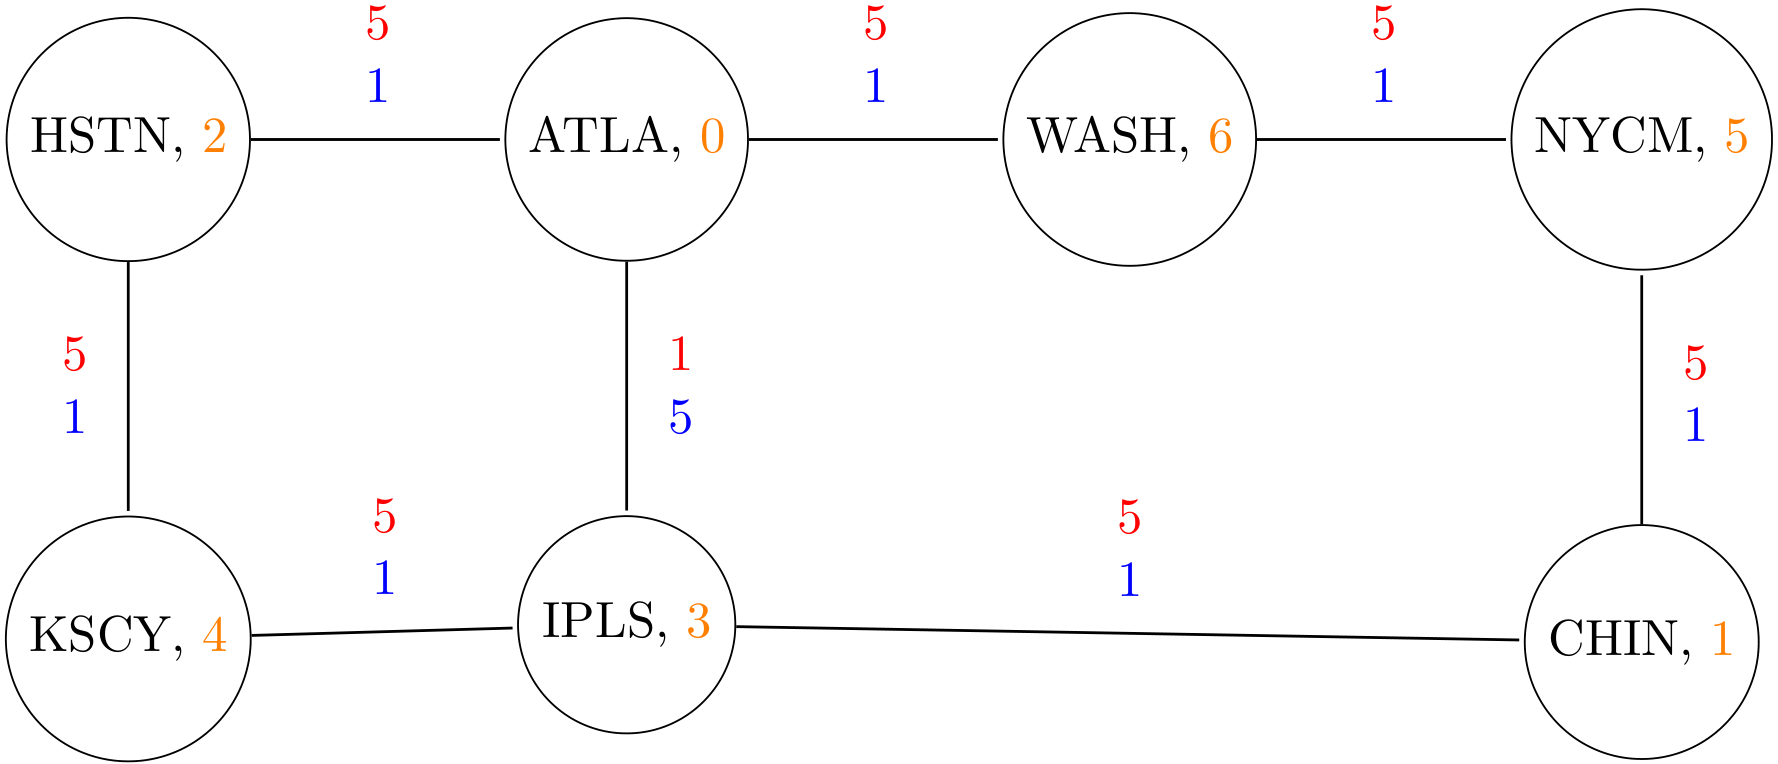
\includegraphics[width=\linewidth]{figures/pouria_simple_topology.png}
\caption{Vereinfachte Netzwerktopologie [Anlehnung an Abilene]. Legende: Kapazit\"aten in rot, Gewichte in blau.}
\label{fig:pouriaSimpleTopology}
\end{figure}
% Das [h] kann weg, dann findet Tabelle automatisch den besten Platz
\begin{table}
\caption{Vereinfachte Anforderungstabelle. Vollst\"andige Tabelle unter \url{https://github.com/fruitiestPunch/FaPro_P2/tree/master/pouria}}
\label{tab:pouriaSimpleTopology}
\begin{tabular}{cccc}
\toprule
$\downarrow$ von, nach $\rightarrow$&IPLS&WASH&$\cdots$\\
\midrule
ATLA & 5 & &\\
IPLS & & 7 & \\
$\vdots$ & & & \\
\bottomrule
\end{tabular}
\end{table}
\section{Replikation}
Im Folgenden werden die Ergebnisse und Einsichten der Replikationen von Gruppe 2 vorgestellt.
\subsection{Replikation zu Projekt 1}
Die Replikation von diesem Projekt war zu Beginn leider etwas schwierig, weil in beiden F\"allen Abh\"angigkeiten fehlten.
Ein gro\ss es Problem beim Replizieren des Deep-Learning-Projekts war, dass sich der Prozess nach einer Weile selbstst\"andig beendet hat.
Die Vermutung liegt nahe, dass der Rechenaufwand so hoch war, dass der Rechner ab einem bestimmten Zeitpunkt den Prozess selbst beendet hat.
Ein weiteres Problem beim Replizieren waren die Fehlermeldungen und Abbr\"uche beim Plotten. 
\begin{figure}
\centering
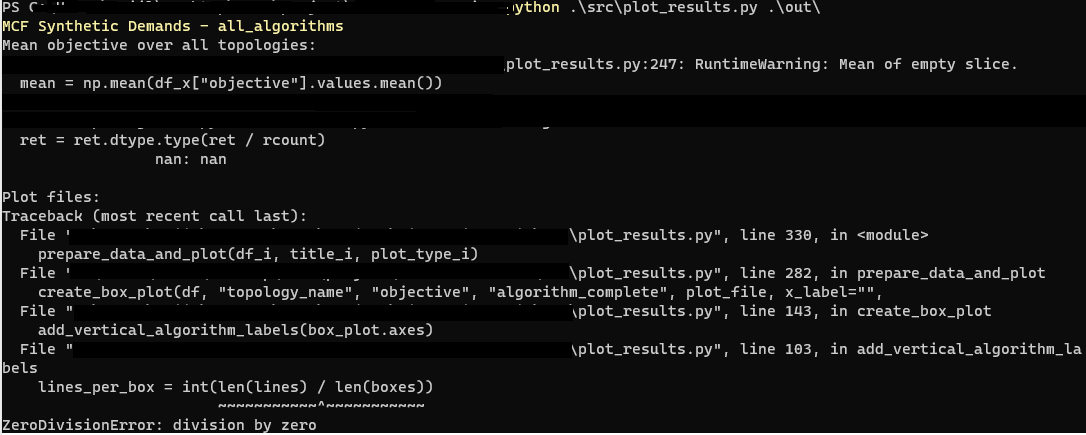
\includegraphics[width=\linewidth]{figures/repl_p1_plottererror.png}
\caption{Plotting-Fehlermeldung im Terminal}
\label{fig:repl_p1_plottererrror}
\end{figure}
Diesem und \"ahnlichen Fehlern sind wir bei unser Bearbeitung ebenfalls begegnet und die Behebung hat sich als au\ss erordentlich schwierig erwiesen, weil dieser "Plottererror" innerhalb einer Python-Bibliothek liegt.
Abbildung \ref{fig:repl_p1_plottererrror} zeigt einen solchen Fehler,
welcher sich hartn\"ackig auch nach einigen Anpassungsversuchen weiterhin erhalten hat.
\subsection{Replikation zu Projekt 2}
Die Replikation des Codes aus Gruppe 2 lief im Allgemeinen problemlos, wie die Abbildungen \ref{fig:repl_p2_daniel2} und \ref{fig:repl_p2_zixiang_10} zeigen.
\begin{figure}
\centering
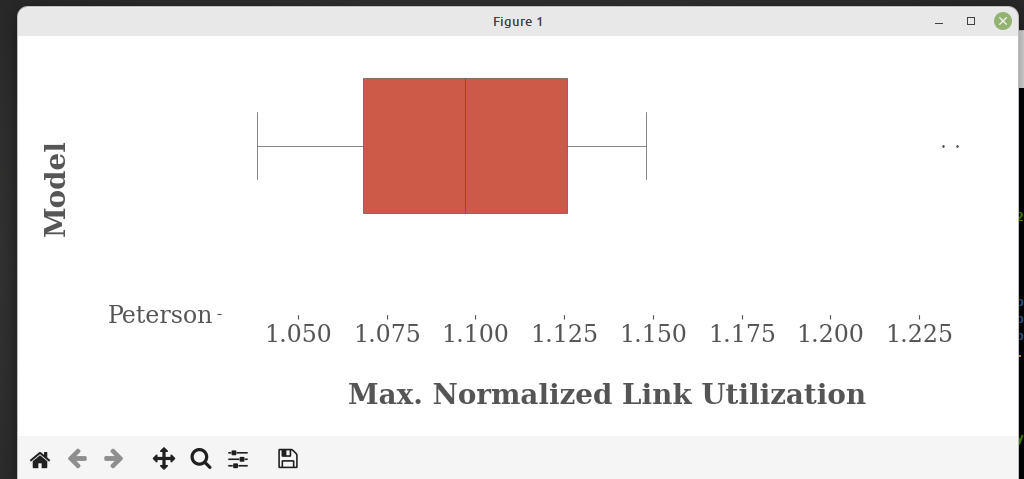
\includegraphics[width=\linewidth]{figures/repl_p2_daniel2.png}
\caption{Ergebnisdiagramm des Codes von Gruppe 2}
\label{fig:repl_p2_daniel2}
\end{figure}
\begin{figure}
\centering
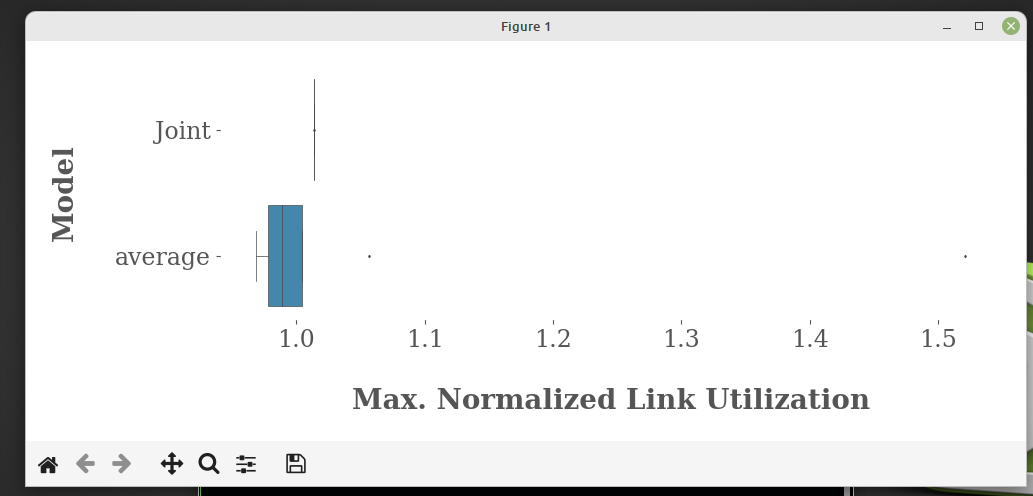
\includegraphics[width=\linewidth]{figures/repl_p2_zixiang_10.png}
\caption{Ergebnisdiagramm des Codes von Gruppe 2}
\label{fig:repl_p2_zixiang_10}
\end{figure}
Ein Problem, welches auch innerhalb unserer Gruppe aufgetaucht ist,
waren die identischen Werte nach Beendigung der \emph{nanonet\_batch.py}-Datei.
Wie bereits in Abschnitt \ref{sec:seq_com_p2} erw\"ahnt, liegt dieses Problem vermutlich an mangelnder Rechenleistung w\"ahrend des Berechnungsprozesses.
Nach wiederholtem Ausf\"uhren des Codes konnte dieses Problem jedoch behoben werden.
\begin{figure}
\centering
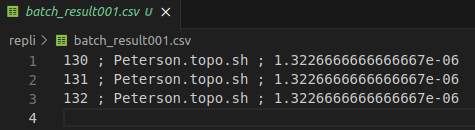
\includegraphics[width=\linewidth]{figures/repl_p2_daniel1.png}
\caption{Ergebnis-CSV-Datei mit identischen MLU-Werten in jeder Zeile}
\label{fig:repl_p2_daniel1}
\end{figure}
\section{Zusammenfassung}
Es kann gesagt werden, dass wir w\"ahrend des Fachprojekts vieles lernen konnten, 
insbesondere Dinge, die nicht notwendigerweise im Stundenplan stehen, 
aber gerade auf der akademischen Laufbahn als Standard angesehen werden.
Das Nachstellen einer wissenschaftlichen Arbeit hat sich als nicht-trivial erwiesen 
und das obwohl diese Arbeit f\"ur ihre hohe Reproduzierbarkeit ausgezeichnet wurde.
Dies l\"asst leider nur auf eine Folgerung schlie\ss en; viele andere wissenschaftlichen Arbeiten lassen sich viel schwerer oder gar nicht nachstellen. 
W\"ahrend des Replizierens der Projekte der anderen Gruppen war es ebenfall \"uberraschend, 
das selbst wenn unsere Gruppen alle an denselbem Hauptprojekt gearbeitet haben 
und theoretisch alle dieselben Pakete verwendeten, 
es manchmal dennoch zu Replikationsschwierigkeiten kam.
Allerdings war es auch eine sch\"one Erfahrung in einer Gruppe an so einem Projekt zu sitzen 
und die Probleme intern sowie mit den anderen Gruppen besprechen zu k\"onnen.
Das hat nicht nur zu einem gr\"o\ss eren Zusammengeh\"origkeitsgef\"uhl gef\"uhrt,
sondern wir haben auch gelernt, kollaborativ gemeinsame Schwierigkeiten zu l\"osen. 
\section{Ausblick}
Aufgrund der relativ kurzen Bearbeitungszeit und den begrenzten Rechenkapazit\"aten unserer eigenen Computer war es etwas schwer, unsere Algorithmen, insbesondere in Projekt 2, auf gro\ss en Topologien zu testen.
Dies kann dazu f\"uhren, dass bestimmt Effekte wie Datenstaus, welche gerade in gro\ss en Topologien auftauchen, in kleinen kaum oder gar nicht vorkommen.

\begin{acks}
Vielen Dank an Marvin f\"ur seine Hilfe und Geduld mit unseren Problemen. Ohne seine Hilfe w\"are das alles in der kurzen Zeit sehr viel schwieriger gewesen.
\end{acks}

\bibliographystyle{ACM-Reference-Format}
\bibliography{fapro_bib}

\appendix
\pagebreak
\section{Zus\"atzliche Abbildungen}
% Das [h] kann weg, dann findet Tabelle automatisch den besten Platz
\begin{figure}
\centering
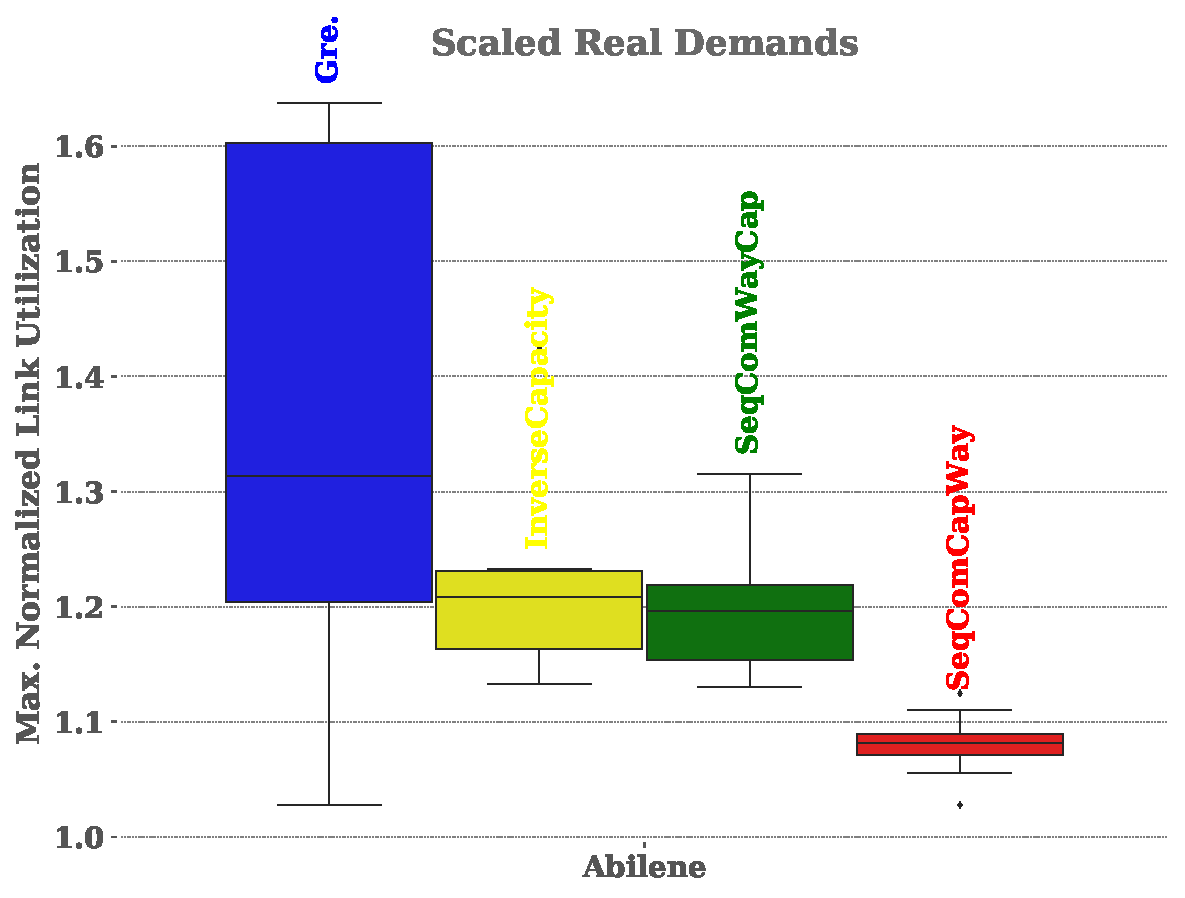
\includegraphics[width=\linewidth]{figures/pouria_real_demands.pdf}
\caption{Vergleich von vier Algorithmen mit realen Anforderungen auf der Abilene-Topologie. Legende: greedy waypoints in blau, inverse capacity in gelb, SeqComWayCap in gr\"un, SeqComCapWay in rot.}
\label{fig:pouriaBoxplotReal}
\end{figure}
% Das [h] kann weg, dann findet Tabelle automatisch den besten Platz
\begin{figure}
\centering
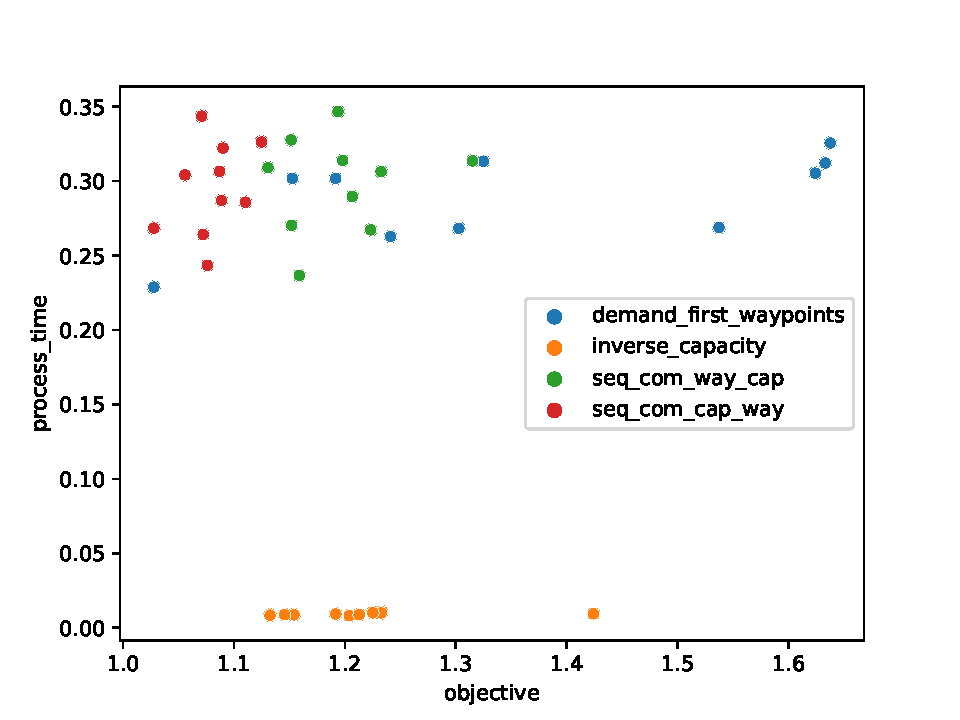
\includegraphics[width=\linewidth]{figures/pouria_colored_scatter_plot_results_real_demands.pdf}
\caption{Vergleich von vier Algorithmen mit syntetischen Anforderungen auf der Abilene-Topologie. Legende: greedy waypoints in blau, inverse capacity in gelb, SeqComWayCap in gr\"un, SeqComCapWay in rot.}
\label{fig:pouriaScatterReal}
\end{figure}
\section{Onlineressourcen}
\label{sec:resouces}
Im Rahmen dieses Fachprojekts wurden drei \"offentliche Repositories als Hauptquellen verwendet. Die ersten beiden Repositories \url{https://github.com/fruitiestPunch/FaPro_P1} und \url{https://github.com/fruitiestPunch/FaPro_P2}, welche \emph{forks} von \url{https://github.com/tfenz/TE_SR_WAN_simulation} und \url{https://github.com/nikolaussuess/TE_SR_experiments_2021} sind. Die dritte Hauptquelle stellt \url{https://github.com/nikolaussuess/nanonet} dar, welche zur Erstellung von vom Projekt les- und interpretierbaren Netzwerktopologiedaten verwendet wurde.
\end{document}